%==============================================================================
% Figure: E6 Dynkin Diagram and Root Structure
% Purpose: Visualize E6 Dynkin diagram and root system properties
% Chapter: Ch03 - Exceptional Lie Groups
% Type: Mathematical
%==============================================================================

\begin{figure}[htbp]
  \centering
  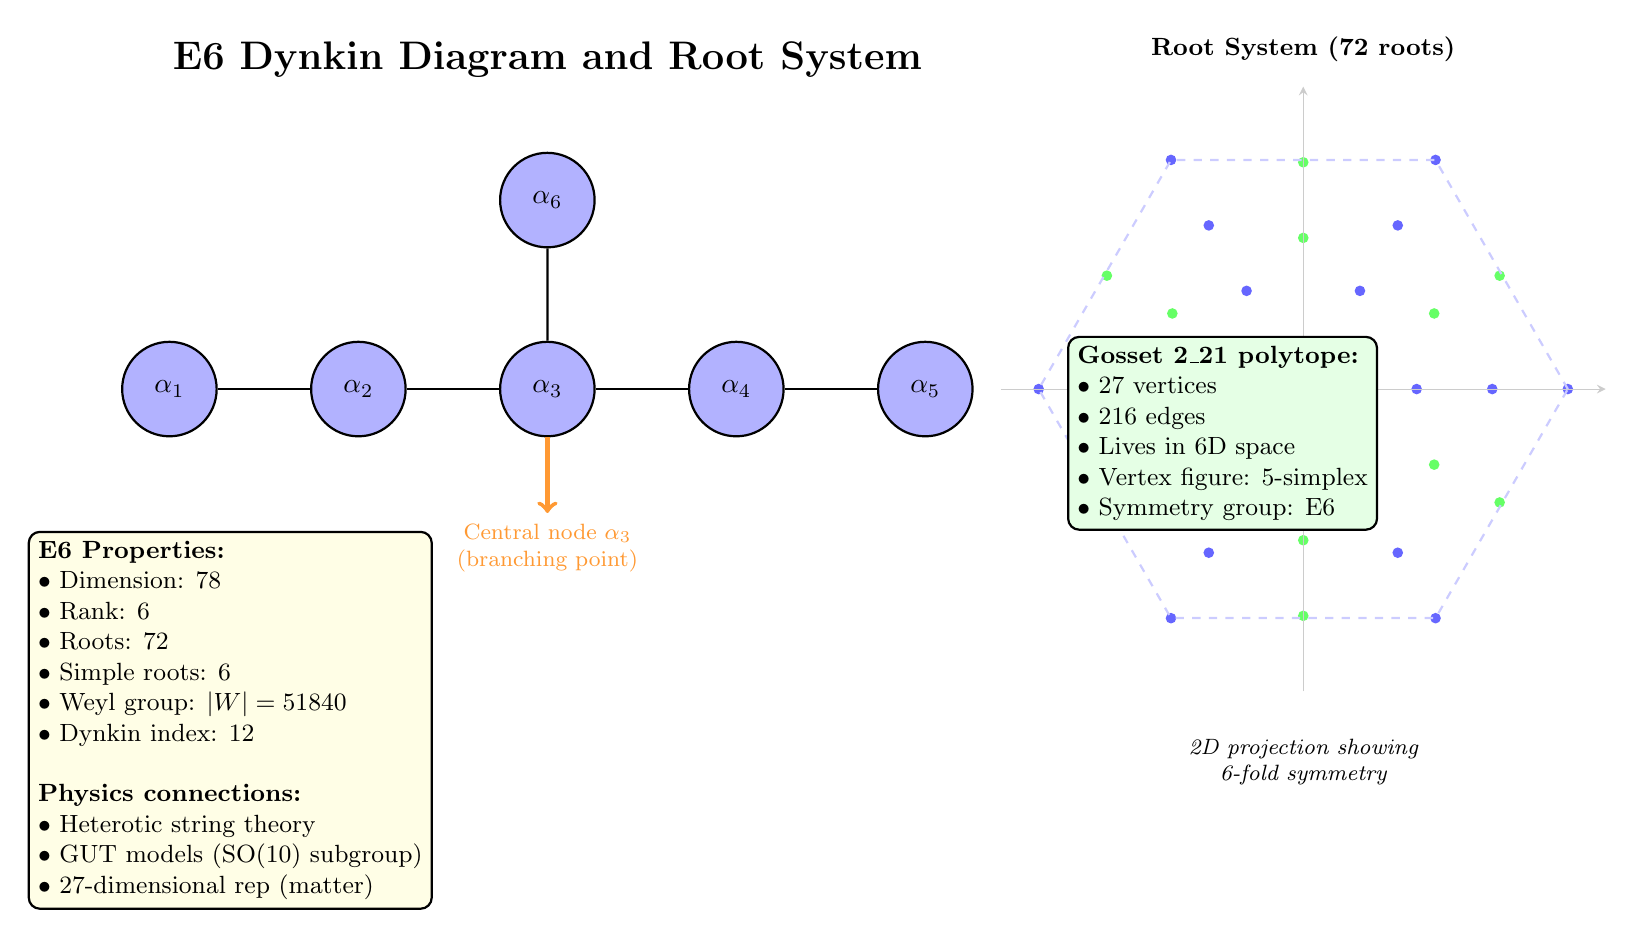
\begin{tikzpicture}[
    scale=1.2,
    node/.style={circle, draw=black, fill=blue!30, thick, minimum size=12mm, font=\bfseries},
    edge/.style={thick, black}
  ]

    % E6 Dynkin diagram: 6 nodes with specific connection pattern
    %     o (alpha_6)
    %     |
    % o---o---o---o---o
    % (1) (2) (3) (4) (5)

    % Horizontal chain nodes
    \node[node] (a1) at (0, 0) {$\alpha_1$};
    \node[node] (a2) at (2, 0) {$\alpha_2$};
    \node[node] (a3) at (4, 0) {$\alpha_3$};
    \node[node] (a4) at (6, 0) {$\alpha_4$};
    \node[node] (a5) at (8, 0) {$\alpha_5$};

    % Branching node
    \node[node] (a6) at (4, 2) {$\alpha_6$};

    % Edges (simple bonds, all equal weight)
    \draw[edge] (a1) -- (a2);
    \draw[edge] (a2) -- (a3);
    \draw[edge] (a3) -- (a4);
    \draw[edge] (a4) -- (a5);
    \draw[edge] (a3) -- (a6);

    % Cartan matrix annotation (partial)
    \node[anchor=north west, align=left, font=\small, draw=black, fill=yellow!10, rounded corners, thick]
      at (-1.5, -1.5) {
      \textbf{E6 Properties:} \\
      $\bullet$ Dimension: 78 \\
      $\bullet$ Rank: 6 \\
      $\bullet$ Roots: 72 \\
      $\bullet$ Simple roots: 6 \\
      $\bullet$ Weyl group: $|W| = 51840$ \\
      $\bullet$ Dynkin index: 12 \\
      \\
      \textbf{Physics connections:} \\
      $\bullet$ Heterotic string theory \\
      $\bullet$ GUT models (SO(10) subgroup) \\
      $\bullet$ 27-dimensional rep (matter)
    };

    % Root system diagram (simplified 2D projection)
    \begin{scope}[shift={(12, 0)}, scale=0.8]
      % Draw a schematic representation of the 72 roots in 2D
      % E6 roots project nicely onto a 2D plane with hexagonal symmetry

      \foreach \r in {1.5, 2.5, 3.5} {
        \foreach \angle in {0, 60, 120, 180, 240, 300} {
          \pgfmathsetmacro\x{\r * cos(\angle)}
          \pgfmathsetmacro\y{\r * sin(\angle)}
          \fill[blue!60] (\x, \y) circle (2pt);
        }
      }

      % Additional roots at intermediate angles
      \foreach \r in {2.0, 3.0} {
        \foreach \angle in {30, 90, 150, 210, 270, 330} {
          \pgfmathsetmacro\x{\r * cos(\angle)}
          \pgfmathsetmacro\y{\r * sin(\angle)}
          \fill[green!60] (\x, \y) circle (2pt);
        }
      }

      % Origin
      \fill[red!70] (0, 0) circle (3pt);

      % Axes
      \draw[->, >=stealth, gray!40] (-4, 0) -- (4, 0);
      \draw[->, >=stealth, gray!40] (0, -4) -- (0, 4);

      % Hexagonal symmetry guide
      \draw[blue!20, thick, dashed] (3.5, 0) -- (1.75, 3.03) -- (-1.75, 3.03) -- (-3.5, 0) -- (-1.75, -3.03) -- (1.75, -3.03) -- cycle;

      \node[anchor=south, font=\small\bfseries] at (0, 4.2) {Root System (72 roots)};
      \node[anchor=north, font=\footnotesize\itshape, text width=3cm, align=center] at (0, -4.5) {
        2D projection showing \\
        6-fold symmetry
      };
    \end{scope}

    % Gosset polytope 2_21 connection
    \node[anchor=south west, align=left, font=\small, draw=black, fill=green!10, rounded corners, thick]
      at (9.5, -1.5) {
      \textbf{Gosset 2\_21 polytope:} \\
      $\bullet$ 27 vertices \\
      $\bullet$ 216 edges \\
      $\bullet$ Lives in 6D space \\
      $\bullet$ Vertex figure: 5-simplex \\
      $\bullet$ Symmetry group: E6
    };

    % Title
    \node[anchor=south, font=\Large\bfseries] at (4, 3.2) {E6 Dynkin Diagram and Root System};

    % Highest root annotation
    \draw[->, ultra thick, orange!80] (a3.south) -- ++(0, -0.8) node[below, font=\footnotesize, align=center] {
      Central node $\alpha_3$ \\
      (branching point)
    };

  \end{tikzpicture}
  \caption{Dynkin diagram and root system for the exceptional Lie algebra $\mathfrak{e}_6$
    (dimension 78). The Dynkin diagram shows 6 simple roots arranged in a characteristic
    branching pattern: a chain of 5 nodes with a 6th node attached to the middle (node 3).
    All edges are simple bonds (no multiple bonds), indicating all roots have equal length.
    The root system contains 72 roots total, which project onto a 2D plane with 6-fold hexagonal
    symmetry (right panel). E6 appears in heterotic string theory compactifications and grand
    unified theories (GUTs). Its fundamental 27-dimensional representation describes matter
    content in certain GUT models. The associated Gosset polytope $2_{21}$ has 27 vertices
    in 6D space, with E6 as its symmetry group.}
  \label{fig:e6-dynkin-diagram}
\end{figure}
